\newcounter{english}
\documentclass{article}

% packages
\usepackage{amsmath, amsthm, thmtools, amsfonts, amssymb, luacode, catchfile, tikzducks, hyperref, ifthen}
\ifcsname c@kobocompile\endcsname
	\usepackage[a5paper, total={1072pt, 1448pt}, margin=10pt, includeheadfoot]{geometry} % set page margins
\else
	\usepackage[a4paper, margin=50pt, includeheadfoot]{geometry}
\fi
\usepackage[shortlabels]{enumitem}
\usepackage[skip=3pt, indent=0pt]{parskip}

% language
\usepackage[bidi=basic, layout=tabular, provide=*]{babel}
\ifcsname c@english\endcsname
	\babelprovide[main, import]{english}
\else
	\babelprovide[main, import]{hebrew}
	\babelprovide{rl}
\fi
%\babelfont{rm}{Libertinus Serif}
\babelfont{rm}[Renderer=Harfbuzz]{Libertinus Serif}
\babelfont{sf}{Libertinus Sans}
\babelfont{tt}{Libertinus Mono}

% style
\AddToHook{cmd/section/before}{\clearpage}	% Add line break before section
\linespread{1.3}
\setcounter{secnumdepth}{0}		% Remove default number tags from sections, this won't do well with theorems
\AtBeginDocument{\setlength{\belowdisplayskip}{3pt}}
\AtBeginDocument{\setlength{\abovedisplayskip}{3pt}}
\graphicspath{ {../images/} }

% operators
\DeclareMathOperator\cis{cis}
\DeclareMathOperator\Sp{Sp}
\DeclareMathOperator\tr{tr}
\DeclareMathOperator\im{Im}
\DeclareMathOperator\re{Re}
\DeclareMathOperator\diag{diag}
\DeclareMathOperator*\lowlim{\underline{lim}}
\DeclareMathOperator*\uplim{\overline{lim}}
\DeclareMathOperator\rng{rng}
\DeclareMathOperator\Sym{Sym}
\DeclareMathOperator\Arg{Arg}
\DeclareMathOperator\Log{Log}
\DeclareMathOperator\dom{dom}
\DeclareMathOperator\supp{Supp}
\DeclareMathOperator\var{Var}
\DeclareMathOperator\cov{Cov}

% commands
%\renewcommand\qedsymbol{\textbf{מש''ל}}
%\renewcommand\qedsymbol{\fbox{\emoji{lizard}}}
\newcommand{\Aa}[0]{\mathcal{A}}
\newcommand{\Bb}[0]{\mathcal{B}}
\newcommand{\CC}[0]{\mathbb{C}}
\newcommand{\Cc}[0]{\mathcal{C}}
\newcommand{\EE}[0]{\mathbb{E}}
\newcommand{\FF}[0]{\mathbb{F}}
\newcommand{\Ff}[0]{\mathcal{F}}
\newcommand{\Ii}[0]{\mathcal{I}}
\newcommand{\Gg}[0]{\mathcal{G}}
\newcommand{\Ll}[0]{\mathcal{L}}
\newcommand{\Mm}[0]{\mathcal{M}}
\newcommand{\NN}[0]{\mathbb{N}}
\newcommand{\Nn}[0]{\mathcal{N}}
\newcommand{\PP}[0]{\mathbb{P}}
\newcommand{\Pp}[0]{\mathcal{P}}
\newcommand{\QQ}[0]{\mathbb{Q}}
\newcommand{\RR}[0]{\mathbb{R}}
\newcommand{\Rr}[0]{\mathcal{R}}
\newcommand{\Ss}[0]{\mathcal{S}}
\newcommand{\TT}[0]{\mathbb{T}}
\newcommand{\Uu}[0]{\mathcal{U}}
\newcommand{\Vv}[0]{\mathcal{V}}
\newcommand{\Ww}[0]{\mathcal{W}}
\newcommand{\ZZ}[0]{\mathbb{Z}}
\newcommand{\acts}[0]{\circlearrowright}
\newcommand{\explain}[2] {
	\begin{flalign*}
		 && \text{#2} && \text{#1}
	\end{flalign*}
}
\newcommand{\maketitleprint}[0]{ \begin{center}
	%\begin{tikzpicture}[scale=3]
	%	\duck[graduate=gray!20!black, tassel=red!70!black]
	%\end{tikzpicture}	
	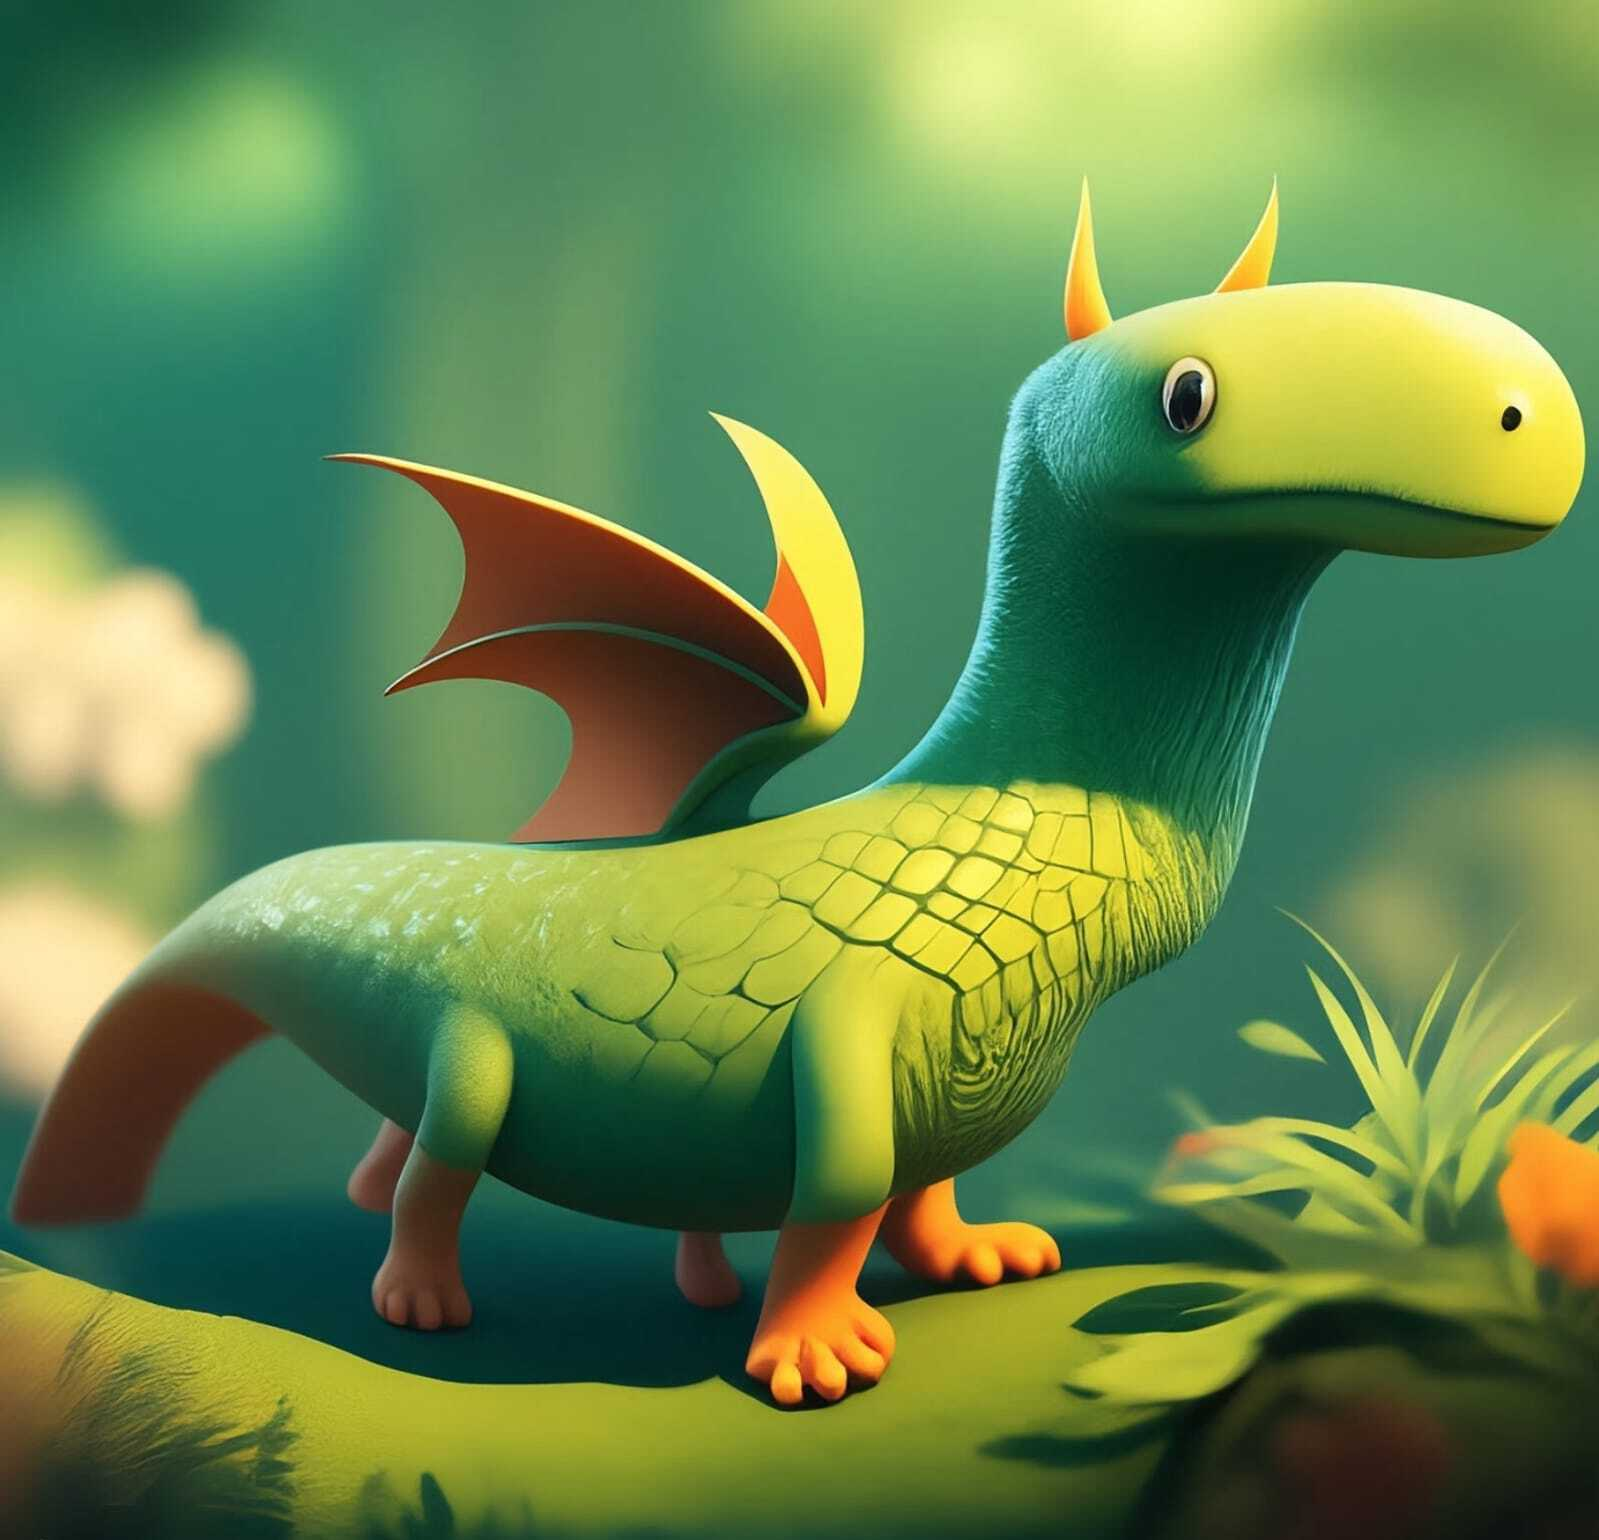
\includegraphics[width=6cm]{cover}
\end{center}
}

% theorem commands
\newtheoremstyle{c_remark}
	{}	% Space above
	{}	% Space below
	{}% Body font
	{}	% Indent amount
	{\bfseries}	% Theorem head font
	{}	% Punctuation after theorem head
	{.5em}	% Space after theorem head
	{\thmname{#1}\thmnumber{ #2}\thmnote{ \normalfont{\text{(#3)}}}}	% head content
\newtheoremstyle{c_definition}
	{3pt}	% Space above
	{3pt}	% Space below
	{}% Body font
	{}	% Indent amount
	{\bfseries}	% Theorem head font
	{}	% Punctuation after theorem head
	{.5em}	% Space after theorem head
	{\thmname{#1}\thmnumber{ #2}\thmnote{ \normalfont{\text{(#3)}}}}	% head content
\newtheoremstyle{c_plain}
	{3pt}	% Space above
	{3pt}	% Space below
	{\itshape}% Body font
	{}	% Indent amount
	{\bfseries}	% Theorem head font
	{}	% Punctuation after theorem head
	{.5em}	% Space after theorem head
	{\thmname{#1}\thmnumber{ #2}\thmnote{ \text{(#3)}}}	% head content

\ifcsname c@english\endcsname
	\theoremstyle{plain}
	\newtheorem{theorem}{Theorem}[section]
	\newtheorem{lemma}[theorem]{Lemma}
	\newtheorem{proposition}[theorem]{Proposition}
	\newtheorem*{proposition*}{Proposition}
	%\newtheorem{corollary}[theorem]{אין חלופה עברית}

	\theoremstyle{definition}
	\newtheorem{definition}[theorem]{Definition}
	\newtheorem*{definition*}{Definition}
	\newtheorem{example}{Example}[section]
	\newtheorem{exercise}{Exercise}[section]

	\theoremstyle{remark}
	\newtheorem*{remark}{Remark}
	\newtheorem*{solution}{Solution}
	\newtheorem{conclusion}[theorem]{Conclusion}
	\newtheorem{notation}[theorem]{Notation}
\else
	\theoremstyle{c_plain}
	\newtheorem{theorem}{משפט}[section]
	\newtheorem{lemma}[theorem]{למה}
	\newtheorem{proposition}[theorem]{טענה}
	\newtheorem*{proposition*}{טענה}
	%\newtheorem{corollary}[theorem]{אין חלופה עברית}

	\theoremstyle{c_definition}
	\newtheorem{definition}[theorem]{הגדרה}
	\newtheorem*{definition*}{הגדרה}
	\newtheorem{example}{דוגמה}[section]
	\newtheorem{exercise}{תרגיל}[section]

	\theoremstyle{c_remark}
	\newtheorem*{remark}{הערה}
	\newtheorem*{solution}{פתרון}
	\newtheorem{conclusion}[theorem]{מסקנה}
	\newtheorem{notation}[theorem]{סימון}
\fi

% Questions related commands
\newcounter{question}
\setcounter{question}{1}
\newcounter{sub_question}
\setcounter{sub_question}{1}

\ifcsname c@english\endcsname
	\newcommand{\question}[1][0]{
		\ifthenelse{#1 = 0}{}{\setcounter{question}{#1}}
		\section{Question \arabic{question}}
		\addtocounter{question}{1}
		\setcounter{sub_question}{1}
	}

	\newcommand{\subquestion}[1][0]{
		\ifthenelse{#1 = 0}{}{\setcounter{sub_question}{#1}}
		\subsection{Part \alph{sub_question}}
		\addtocounter{sub_question}{1}
	}
\else
	\newcommand{\question}[1][0]{
		\ifthenelse{#1 = 0}{}{\setcounter{question}{#1}}
		\section{שאלה \arabic{question}}
		\addtocounter{question}{1}
		\setcounter{sub_question}{1}
	}

	\newcommand{\subquestion}[1][0]{
		\ifthenelse{#1 = 0}{}{\setcounter{sub_question}{#1}}
		\subsection{סעיף \localecounter{letters.gershayim}{sub_question}}
		\addtocounter{sub_question}{1}
	}
\fi

% import lua and start of document
\directlua{common = require ('../common')}

\GetEnv{AUTHOR}

% headers
\author{\AUTHOR}
\date\today

\title{Solution to Final Exercise --- Logic Theory (2), 80424}

\DeclareMathOperator{\PA}{PA}
\DeclareMathOperator{\Coll}{Coll}
\DeclareMathOperator{\Ind}{Ind}
\DeclareMathOperator{\Sat}{Sat}
\DeclareMathOperator{\pr}{Pr}
\DeclareMathOperator{\sent}{sent}
\DeclareMathOperator{\form}{form}
\DeclareMathOperator{\val}{Val}
\DeclareMathOperator{\sat}{Sat}
\DeclareMathOperator{\term}{term}
\DeclareMathOperator{\sk}{Sk}
\DeclareMathOperator{\FV}{FV}

\begin{document}
\maketitle
\maketitleprint[yellow]

\question{}
\subquestion{}
Let $U \subseteq \Pp(\NN)$ be a non-principal ultrafilter, let $\langle \Mm_n \mid n < \omega \rangle$ be a sequence of $L$-structures, and $\Mm = \prod_{n < \omega} \Mm_n / U$. \\
We will show that for every countable consistent set of formulas $\Gamma(x)$ with parameters from $M$ is realized in $\Mm$, namely that $\Mm$ is countably saturated.
\begin{proof}
	$\Gamma(x)$ is countable, then we notate $\Gamma = \{ \gamma_n(x) \mid n < \omega \}$, and define $\Sigma_n(x) = \{ \gamma_m(x) \mid m < n \}$.
	$\langle \Sigma_n \mid n < \omega \rangle$ is increasing sequence of formulas.
	For any $n$, $\Sigma_n$ is realized, and let $f_n \in \prod_{i < \omega} M_i$ be a function such that $\Mm \models \Sigma_n([f_n])$.
	Then $a_n = \{ j < \omega \mid \Mm_n \models \Sigma_n(f_n(j)) \} \in U$. \\
	Filters are closed to intersection, then we assume without loss of generality that $a_{n + 1} \subseteq a_n$, otherwise we could have defined,
	\[
		g_{n + 1}(i) = \begin{cases}
			f_{n + 1}(i) & i \in a_n \\
			c_n & \text{otherwise}
		\end{cases}
	\]
	where $c_n \in M_n$ is some arbitrary constant value.

	We now take $a = \bigcap_{n < \omega} a_n$, if $a \in U$ then we can define $f \in \prod_{i < \omega} M_i$ such that $\forall n \in a,\ f(n) \in \{ f_i(n) \mid i \in a \}$ and conclude the claim.
	Otherwise $a \notin U$, then let $[f] \in M$ such that for $n \in a$, $f(n) = f_k(n)$ for the maximal $k < \omega$ such that $n \in a_k$.
	For any $\Sigma_n$ we get that $\Mm \models \Sigma_n([f])$, therefore $\Mm \models \Gamma([f])$ as well.

	We can also prove the claim using part c by showing that $U$ is not $\sigma$-complete. \\
	We define $a_n = \omega \setminus \{ n \}$, $U$ is not principal then $\{ n \} \notin U$ and $a_n \in U$.
	But $\bigcap_{n < \omega} a_n = \emptyset \notin U$.
\end{proof}

\subquestion{}
We define $\sigma$-complete ultrafilter $U$ as an ultrafilter that is closed under countable intersections. \\
Let $U$ be some $\sigma$-complete ultrafilter, $L = \{ = \}$, $\Mm = {(\NN, =)}^I / U$ for some index set $I$. \\
We will show that $|M| = \omega$ and deduce that $\Mm$ is not countably saturated.
\begin{proof}
	Let $\varphi_N$ be the sentence that there are at least $N$ unique elements,
	\[
		\varphi_N = \exists x_0 \ldots \exists x_{N - 1}\ \left( \bigwedge_{m, n < N} x_n \ne x_m \right)
	\]
	$(\NN, =) \models \varphi_N$ for every $N$ as $|\NN|$ is not finite.
	By Łoś theorem we deduce that $|M| \ge \omega$. \\
	Define $C_x = {\{ x \}}^I$ the constant function, we will show that for every $[f] \in M$ there is $n < \omega$ such that $[f] = [C_n]$.
	Note that this is equivalent to the claim that $\{ j < \omega \mid f(j) = n \} \in U$.
	Towards a contradiction, we assume that $a_n = \{ j < \omega \mid f(j) \ne n \} \in U$ for all $n < \omega$.
	Take $a = \bigcap_{n < \omega} a_n$, $U$ is $\sigma$-complete thus $a \in U$.
	It follows that $f(j) \ne n$ for all $j \in a, n < \omega$, a contradiction to $f$ being total function.

	It follows that $|M| = \omega$ and $\Mm \cong (\NN, =)$.
	In particular we can notate $M = \{ m_i \mid i < \omega \}$ and,
	\[
		\psi_n(x)
		= x \ne m_n
	\]
	If $\Gamma(x) = \{ \psi_n \mid n < \omega \}$ then $\Gamma$ cannot be realized, and accordingly $\Mm$ is not countably saturated.
\end{proof}

\subquestion{}
We will show that if $U$ is an ultrafilter on some indices set $I$ such that $U$ is not $\sigma$-complete and $\langle \Mm_i \mid i \in I \rangle$ sequence of models,
then $\Mm = \prod_{i \in I} \Mm_i / U$ is countably saturated.
\begin{proof}
	By $\sigma$-incompleteness we can assume that there is decreasing chain $\langle u_n \mid j < \omega \rangle \subseteq U$ such that $\bigcap_{n < \omega} u_n \notin U$.
	We can assume without loss of generality that $\bigcap u_n = \emptyset$ as $I \setminus \bigcap u_n \in U$ and therefore we can take $u_n \setminus \bigcap u_m$.

	Let $\Gamma(x)$ be countably realized set of formulas.
	By countability let us denote $\Gamma(x) = \{ \gamma_n \mid n < \omega \}$.
	For every $N < \omega$ we also define $\Gamma_N = \{ \gamma_n \mid n < N \}$.
	Then $\Gamma_N$ is finite set of formulas, by our assumption is realized by some $[f_N] \in M$.
	We can take $f_N$ such that,
	\[
		a_N
		= \{ j \in I \mid \Mm_j \models \Gamma_N(f_N(j)) \}
		\subseteq \{ j \in I \mid \Mm_j \models \Gamma_N(f_M(j)) \}
	\]
	where $M < N$ by finite intersections.
	The sequence $\langle a_n \mid n < \omega \rangle \subseteq U$ is decreasing.
	Let us take $U_n = u_n \cap a_n$ for every $n$, clearly $U_n \in U$.
	Note that for every $i \in I$ there is maximal $n < \omega$ such that $i \in U_n$ as $\bigcap_{n < \omega} U_n = \emptyset$, and let us define $f(i) = f_n(i)$.
	Indeed $f \in M$ and,
	\[
		\Mm \models \gamma_n([f])
		\iff \{ j \in I \mid \Mm_j \models \gamma_n(f(j)) \} \in U
		\impliedby \{ j \in I \mid \Mm_j \models \gamma_n(f_n(j)) \} \in U
	\]
	but the latter holds directly by the definition of $f$, then,
	\[
		\Mm \models \Gamma([f])
	\]
	as required.
\end{proof}

\question{}
We will show that the following are equivalent,
\begin{enumerate}
	\item The axiom of choice
	\item
		\begin{enumerate}
			\item The ultrafilter lemma: Every filter extends to an ultrafilter
			\item Alternative version of Łoś theorem: If $\Mm$ is an $L$-structure and $U$ is an ultrafilter on indices set $I$, then for any sentence $\varphi$, $\Mm^I / U \models \varphi \iff \Mm \models \varphi$
		\end{enumerate}
\end{enumerate}
\begin{proof}
	$1 \implies 2$.
	We saw in class that the ultrafilter lemma is directly deduced from Zorn's lemma, which is equivalent to the axiom of choice;
	Let $D$ be a filter, we define the order $X = \langle \{ D \subseteq F \subseteq \Pp(I) \mid F \text{ is a filter} \}, \subseteq \rangle$.
	$X$ is clearly not empty as $D \in X$. Let $C \subseteq X$ be a chain, and let $D_C = \bigcup C$.
	Then $D_C$ is a filter and in particular $D \subseteq D_C$, then $D_C \in X$ and $F \subseteq D_C$ for all $F \in C$.
	By Zorn's lemma there is maximal element $U_D \in X$, namely $U_D \subseteq F$ implies that $U_D = F$ for all $F \in X$. \\
	It reminds to show that maximal filter is an ultrafilter, then let us assume in contradiction that it is not, meaning that there is $A \subseteq I$ such that $A \notin U_D$ as well $I \setminus A \notin U_D$.
	We can define $U = \langle U_D \cup \{ A \} \rangle$, this is a filter such that $U_D \subsetneq U$, a contradiction to $U_D$ being maximal.

	As for the alternative version of Łoś theorem, it is derived from the general version for ultra-powers.
	While we will not recite the whole proof, we will note where it uses choice.
	The axiom of choice is being used in the proof at induction step for quantifiers, specifically to get a witness to global quantifiers.

	$2 \implies 1$.
	Let $A$ be some set such that $\emptyset \notin A$, and let us assume toward a contradiction that there is no choice function $A \to \bigcup A$.
	We define $S \subseteq \Pp(A)$ the set of all subsets of $A$ that do have choice function.
	In particular $\emptyset \in S$ as $\emptyset \to \bigcup \emptyset = \emptyset$ is witnessed by $\emptyset$.

	Let $B \in S$ and $f : B \to \bigcup B$ choice function, namely $\forall b \in B,\ f(b) \in b$.
	For every $B' \subseteq B$ consider $f' = f \restriction B'$.
	$f'(b) \in b$ directly by $f$'s definition, then $\rng f' \subseteq \bigcup B'$.
	We conclude that $B' \in S$, meaning $S$ is closed under subsets.

	Let $B, C \in S$, we will show that $B \cup C \in S$ as well.
	We will assume that they are disjoint, as otherwise we can take $B' = B \setminus C \subseteq B$ by closeness to subsets.
	if $f : B \to \bigcup B, g : C \to \bigcup C$ such that $\forall b \in B, c \in C,\ f(b) \in b, g(c) \in c$, then $h = f \cup g$ is well-defined function,
	as for each $x \in \dom h$, either $x \in B$ or $x \in C$.
	Also $f(x) \in B \lor f(x) \in C$ then $f(x) \in B \cup C$.
	We deduce that $S$ is closed to finite unions by induction.

	We define $D = \Pp(A) \setminus S$, the collection of subsets such that there is no choice function over them. In particular by our assumption $A \in D$.
	By inversion we conclude that $D$ is closed under super-sets and finite intersections, as well $\emptyset \notin D$, then $D$ is a filter.
	Using the ultrafilter lemma we define $D \subseteq U$ an ultrafilter extending $D$.

	Let us define $\Mm = \langle \bigcup A, R \rangle$ such that $\langle x, y \rangle \in R^\Mm \iff \exists a \in A,\ x, y \in a$.
	We assume that $a \cap b = \emptyset$ for all $a, b \in A$ as well.
	Then $R^\Mm$ is equivalency relation, and therefore $R^{\Mm^A / U}$ is as well.
	Let $B \in S$ be some non-trivial set and let $g : B \to M$ be choice function.
	then $[g] \in \Mm^A / U$.
	We assumed that $B$ is not trivial then there are $x, y \in A$, $\langle g(x), g(y) \rangle \notin R^{\Mm}$.
	But then it immediately follows that $\langle [g], [c_{g(x)}] \rangle, \langle [g], [c_{g(y)}] \rangle \in R^{\Mm^A / U}$ in contradiction to $\langle [c_{g(x)}], [c_{g(y)}] \rangle \notin R^{\Mm^A / U}$.
\end{proof}

\question{}
We will show that if $t$ is a term that does not contain the variable $v$, and $\varphi \in \Sigma_0^0$,
then $\forall v \le t\ \varphi$ is $\Sigma_0^0$-formula as well.
We will conclude that $\Sigma_0^0$ is closed under bounded quantification with general terms.
\begin{proof}
	Let $\Sigma_0'$ be the closure of the atomic formulas under boolean operations and term-bounded quantifiers.
	Let $\varphi \in \Sigma_0'$, and $t$ is substitutable by $v$ then $\varphi_t^v \in \Sigma_0'$, this can be proved by induction over the structure of $\varphi$.
	Let $q : \Sigma_0' \to \NN$ be count function for quantifiers on a given formula, in particular $q(\varphi) = q(\varphi_t^v)$.
	
	We will show by full induction over $q(\varphi)$ that for any $\varphi \in \Sigma_0'$ also $\varphi \in \Sigma_0^0$.
	The case $q(\varphi) = 0$ is trivial, as $\varphi$ is quantifier-free, thus $\varphi \in \Sigma_0^0$. \\
	Let us assume that for some $q$ the claim holds for any $q' < q$ and will show that it also holds for $q$.
	We will show it using induction over the structure of $\varphi$.
	For the case of atomic formula $\psi$ the claim is trivial as $q(\psi) = 0$.
	The case of negation and binary operations is deriving from closure of $\Sigma_0^0$ to binary operations.
	It remains to show the case $\varphi = \forall v \le t\ \psi$ for $q(\psi) = q - 1$.

	We will show this claim by induction over the structure of $t$.
	For $t = 0, 1$ or $t = w$ for some variable $w \ne v$, the claim holds by the definition of $\Sigma_0^0$.
	For $t = t_0 + t_1$,
	\[
		\forall v \le t\ \psi
		\equiv \forall v_0 \le t_0 \forall v_1 \le t_1\ \psi_{v_0 + v_1}^v
	\]
	and therefore by the induction hypothesis and the first claim we get $\forall v \le t_0 + t_1\ \psi \in \Sigma_0^0$.
	The case of multiplication symbol is identical.

	We have shown that $\varphi \in \Sigma_0' \implies \varphi \in \Sigma_0^0$, or equivalently that $\Sigma_0' \subseteq \Sigma_0^0$,
	meaning that $\Sigma_0^0$ is closed under term-bounded quantifiers.
\end{proof}

\question{}
Let $T$ be a theory.
We will show that the following are equivalent.
\begin{enumerate}
	\item $T$ is axiomatizable
	\item $T$ is recursively-enumerable
	\item There is a recursively-enumerable set $\Sigma$ such that $\cl \Sigma = T$
\end{enumerate}
\begin{proof}
	$1 \implies 2$.
	$T$ is a theory, meaning that $T = \cl T$, and by the assumption that it is axiomatizable there is $\Sigma$ recursive set of sentences such that $T = \cl \Sigma$.
	We proved in class that $\pr(x, y)$ is a recursively-enumerable function,
	where it holds if and only if $x$ is a Gödel number for set of recursively-enumerable formulas and $y$ is Gödel number for formulas $\varphi$, and $\Sigma \models \varphi$.
	By our definition,
	\[
		T = \cl_{\models} \Sigma = \{ \lceil \varphi \rceil \mid \varphi \in \sent_{L_{\PA}}, \pr(\lceil \Sigma \rceil, \lceil \varphi \rceil) \}
	\]
	If we define $f(n) = \pr(\lceil \Sigma \rceil, n)$ we get $T = \dom f$ and by recursively-enumerable formulas equivalencies lemma, it follows that $T$ is recursively-enumerable.

	$2 \implies 3$.
	$T$ is a theory, then $\cl_{\models} T = T$, we define $\Sigma = T$, it follows that $\Sigma$ is recursively-enumerable and $\cl \Sigma = T$.

	$3 \implies 1$.
	Let $f$ be recursive function such that $\dom f = \Sigma$ for recursively-enumerable $\Sigma$, $\cl \Sigma = T$.
	Notice that if $f(n)$ is defined then $\pr(\lceil \Sigma \rceil, n)$ is also defined and returns $1$, then let us assume that $f(n) = \pr(\lceil \Sigma \rceil, n)$.
	We also know that $g : \NN \to \{ 0, 1 \}$ such that $g(n) = 1 \iff \exists \varphi \in \sent_{L_{\PA}},\ n = \lceil \varphi \rceil$ is full recursive function.
	Then $h(n) = f(g(n) \cdot n)$ is recursive function such that $T = h^{-1}(\{ 1 \})$, and witnessing $T$ being axiomatizable.
\end{proof}

\question{}
\subquestion{}
We will show that if $f : \NN^k \to \NN$ is primitive-recursive function then there is a $\Sigma_1$-formula $\varphi(x_0, \ldots, x_{k - 1}, y)$ defining $f$,
such that $\PA \vdash \forall \bar{x} \exists y\ \varphi(\bar{x}, y)$.
\begin{proof}
	We defined primitive-recursive functions in such way that they are recursive in particular, and then proved that every recursive function is $\Sigma_1^0$.
	Let us define $\varphi(\bar{x}, y) = \exists z \psi(\bar{x}, y, z)$ for $\psi \in \Sigma_0$.
	It is clear that $\varphi$ is $\Sigma_1$-formula such that $\varphi(\bar{x}, y) \iff f(\bar{x}) = y$, and thus it is suffices to show that $\PA$ proves that $f$ is total.

	In the proof of the claim from class that we used, we could also prove that the formula is total in $\PA$,
	as for constant and successor functions the claim is trivial in $\PA$, for composition it is immediate from witness choosing, and for closure to primitive recursion it follows from totality of the recursive functions.
\end{proof}

\subquestion{}
We will show that the above claim does not hold for general recursive functions.
\begin{proof}
	Let us assume for contradiction that indeed the claim holds for general total recursive functions.
	Let $\sigma : \NN \to \NN$ be function such that $\sigma(\lceil \varphi \rceil) = \lceil \lnot \varphi \rceil$ and constant otherwise.
	$\sigma$ is primitive-recursive and total, and by Roger's fixed point theorem there is $e \in \NN$ such that,
	\[
		\forall x,\ U(e, x) = U(\sigma(e), x)
	\]
	We notate $f : \NN \to \NN$ as the recursive function,
	\[
		f(x) = y
		\iff \psi(x, y),\ e = \lceil \psi \rceil
	\]
	then,
	\[
		\forall x,\ 
		U(e, x)
		= f(x)
		= 1 \dot{-} f(x)
		= U(\lceil \lnot \psi \rceil, x)
	\]
	then $f$ is nowhere defined,
	\[
		\hat{\NN}
		\not\models \exists x \exists y\ \psi(x, y)
		\iff \hat{\NN}
		\models \forall x \forall y\ \lnot \psi(x, y)
	\]
	Meaning that $\lnot \psi$ is total recursive relation and by our assumption also provably total.

	This is wrong.
\end{proof}

\question{}
Assuming that $\Mm \models \PA$, such that $c \in M$ is non-standard, and let us define $N = \bigcup_{n \in \NN} \{ x \in M \mid x \le^\Mm c^n \}$. \\
We will show that $\Nn \subseteq \Mm$ and that $\Nn \not\models \PA$.
\begin{proof}
	Let $x, y \in N$, we will show that $x + y, x \cdot y \in N$ as well.
	Consider $m \in \NN$ such that $x, y \le c^m$, there must be such $m$ as $\le^\Mm$ is linear.
	It follows that,
	\[
		x + y
		\le c^m + c^m
		= 2 \cdot c^m
		\le c \cdot c^m
		= c^{m + 1}
	\]
	In particular for $y = 1$ we get that $S(x) \in N$.
	We can also see that,
	\[
		x \cdot y
		\le c^m \cdot c^m
		\le c^{2m}
	\]
	Therefore $S(x), x + y, x \cdot y \in N$, meaning that it is a set closed to functions of $\Mm$, we conclude that $\Nn \subseteq \Mm$.

	Let us define the partial function $H : \NN^3 \to \NN$
	\[
		H(n, x, k)
		= x \cdot k
	\]
	and $G = c_1$, then by induction scheme there exists primitive-recursive function $F : \NN^2 \rightharpoonup \NN$ defined by,
	\[
		F(x, 0) = 1,
		\quad
		F(x, n + 1)
		= x \cdot F(n)
	\]
	This is a primitive-recursive from definition therefore it is total, and we denote $x^n = F(x, n)$ for all $x$ and $n$.
	In particular, consider $e = c^c$, this element fulfills $e \in M$, we will show that $e \notin N$.

	the function $F$ fulfills $\PA \models n < m \implies x^n < x^m$ for any $x > 1$.
	The proof is by fixation of $n$, induction over $m$ and then induction over $n$.
	We start by showing that $x^n < x^{S(n)}$, as for $n = 0$ we get $1 < x$ and if $x^n < x^{S(n)}$ then $x \cdot x^n < x \cdot x^{S(n)} \iff x^{S(n)} < x^{S(S(n))}$.
	We can now fix $n$ and prove that $x^n < x^m$ for all $n < m$.
	This time we use $m = S(n)$ as the recursion base, this was proven already.
	The step is identical to the first case.
	We infer from induction scheme that indeed $n < m \implies x^n < x^m$.

	$c \in M$ is non-standard, then $\underline{n} < c$ for all $n \in \hat{\NN}$, it is implied that $c^n < c^c = e$ for all $n$.
	If $x \in N$, then there exists $n \in \hat{\NN}$ such that $x \le c^n < c^{S(n)} < c^c = e$, meaning that $x < e$ for all $x \in N$, as a result $e \notin N$.

	We assume in contradiction that $\Nn \models \PA$, then $F$ is definable and primitive-recursive over $\Nn$.
	We also know that $c \in N$ as $c \le^\Mm c^1$, then $d = F^\Nn(c, c)$ fulfills that $d \in N$ but $\Nn \subseteq \Mm$ and $F^\Nn(c, c) = F^\Mm(c, c) = e \notin N$, a contradiction.
\end{proof}

\question{}
Let $L$ be some language such that it has Gödel numbering.
Let $X$ be a family of sentences in $L$, and,
\begin{align*}
	& \sat(X)
	= \{ \lceil \varphi \rceil \mid \varphi \in X, \exists \Mm,\ \Mm \models \varphi \} \\
	& \sat_{\infty}(X)
	= \{ \lceil \varphi \rceil \mid \varphi \in X, \varphi \text{ has an infinite model} \} \\
	& \val(X)
	= \{ \lceil \varphi \rceil \mid \varphi \in X \land \models \varphi \}
\end{align*}

For this question we assume that $X$ is recursive.
\subquestion{}
We will show that $\sat(X)$ is recursive if and only if $\val(\lnot X)$ is recursive and $\sat(\lnot X)$ is recursive if and only if $\val(X)$ is recursive.
\begin{proof}
	Assume that $\sat(X)$ is recursive, then $X \setminus \sat(X)$ is recursive as well, and by definition $\varphi \in X \setminus \sat(X)$ if there is no model that satisfy $\varphi$.
	But this is exactly $\val(\lnot X)$, as it is the set of sentences such that a sentence $\varphi$ is in $\val(X)$ if $\lnot \varphi$ is tautology, meaning that $\varphi \equiv_{\operatorname{tau}} \perp$.

	Let us assume that $\val(\lnot X)$ is recursive.
	We deduce that $X \setminus \val(X)$ is recursive as well, and yet again by direct definition it is exactly $\sat(X)$.

	The last part of the claim follows from the first part and the fact that $\lceil \varphi \rceil \to \lceil \lnot \varphi \rceil$ is recursive map.
\end{proof}

\subquestion{}
We will show that if $\sat_{\infty}(X)$ is recursive, then $\sat(X)$ is recursive as well.
\begin{proof}
	We notate $\sat_{< \infty}(X) = \{ \lceil \varphi \rceil \in X \mid \exists \Mm \models \varphi, |M| < \infty \}$ the set of sentences of $X$ that are right in some finite model.
	$\sat(X) = \sat_{< \infty}(X) \cup \sat_{\infty}(X)$, and we know that finite union of recursive sets is recursive, then it suffices to show that $\sat_{< \infty}(X)$ is recursive set.
	In the previous course we had shown that there is an embedding between finite models of a countable language and sentences, up to model isomorphism.
	We also saw an algorithm to build such sentences, and can enumerate through it,
	meaning that we can assume that there is $m : \NN \to \NN$ function such that if $\Mm$ a model of $L$ then exists $i \in \NN$ such that $m(i) = \lceil \varphi \rceil$ for $\Mm \models \varphi$.

	By our definition of $\sat_{< \infty}(X)$, an element $n \in \NN$ fulfills $n \in \sat_{< \infty}(X)$ if and only if $\exists i,\ m(i) \models \varphi$, or by using Gödel numbers,
	\[
		\exists i \pr(m(i), n)
		\iff n \in \sat_{< \infty}(X)
	\]
	We can now define $\psi_0(x) = x \in \sat_{\infty}(X) \lor \exists i \pr(m(i), x)$, this is a $\Sigma_1^0$ formula, but it is not clear that it is $\Pi_1^0$ as well.

	$x \notin \sat(X)$ if and only if $x \in \val(\lnot X)$ by the previous part, then $\psi_1(x) = \lnot \pr(x, \lceil \perp \rceil)$ fulfills,
	\[
		\psi_1(x)
		\iff \lnot (x \in \val(\lnot X))
		\iff \lnot (x \notin \sat(X))
		\iff x \in \sat(X)
	\]
	$\psi_1$ is $\Sigma_1^0$ formula and therefore $\lnot \psi_1$ is $\Pi_1^0$. \\
	But it is implied that $\psi_0 \equiv \psi_1$, in particular $\psi_0 \in \Delta_1^0$.
	We deduce that $\psi_0$ defining recursive set, and that this set is exactly $\sat(X)$.
\end{proof}

\question{}
Assume that $L$ is some language and $\varphi(x, y_0, \ldots, y_{k - 1})$ is some formula and that $\Mm$ is an $L$-structure,
A function $f : M^k \to M$ is called \textit{Skolem function for $\varphi$} if for every $a_0, \ldots, a_{k - 1} \in M$,
\[
	\Mm \models \exists x\ \varphi(x, a_0, \ldots, a_{k - 1})
	\implies \Mm \models \varphi(f(a_0, \ldots, a_{k - 1}), a_0, \ldots, a_{k - 1})
\]
A theory $T$ is said to \textit{has a built-in Skolem functions} if for every such formula $\varphi$ there is a term in the language, \\
$t_{\varphi}(y_0, \ldots, y_{k - 1})$, such that $t_\varphi^\Mm$ is a Skolem function for $\varphi$ for any $\Mm \models T$.

\subquestion{}
We will show that if $T$ has a built-in Skolem functions, then $T$ has quantifier elimination,
meaning that for every formula $\psi(x_0, \ldots, x_{n - 1})$ there is a quantifier free formula $\psi'(x_0, \ldots, x_{n - 1})$ such that $T \vdash \forall \bar{x} (\psi \leftrightarrow \psi')$.
\begin{proof}
	The proof is by induction over the structure of the formula.
	For atomic formulas the claim is trivial, as there are no quantifiers in such formulas.
	In the same meaner, binary operations and $\lnot$ preserve quantifier-free formulas.

	We move to the case of existential quantifiers.
	Assume that $\varphi(x_0, \ldots, x_{n - 1}) = \exists v\ \psi(v, x_0, \ldots, x_{n - 1})$, for $\psi$ quantifier-free formula.
	$T$ has built-in Skolem function to $\psi$, $t = t_{\psi}(x_0, \ldots, x_{n - 1})$, such that for $a_0, \ldots, a_{n - 1} \in M$,
	\[
		\Mm \models \varphi(a_0, \ldots, a_{n - 1})
		\implies \Mm \models \psi(t^\Mm(a_0, \ldots, a_{n - 1}), a_0, \ldots, a_{n - 1})
	\]
	It follows that also,
	\[
		\Mm \models \varphi(a_0, \ldots, a_{n - 1}) \to \psi(t^\Mm(a_0, \ldots, a_{n - 1}), a_0, \ldots, a_{n - 1})
	\]
	By defining $\varphi' = \psi_t^v$, and the fact that $\bar{a}$ is arbitrary,
	\[
		\Mm \models \forall \bar{x} (\varphi \to \varphi')
	\]
	It is trivial that $\Mm \models \forall \bar{x} (\varphi' \to \varphi)$ then,
	\[
		\Mm \models \forall \bar{x} (\varphi \leftrightarrow \varphi')
	\]
	This holds for any $\Mm \models T$, then by the completeness theorem, $T \vdash \forall \bar{x} (\varphi \leftrightarrow \varphi')$.
\end{proof}

\subquestion{}
We will show that if $T$ has built-in Skolem functions and $\Mm \models T$, then any $\Nn \subseteq \Mm$ is an elementary substructure.
\begin{proof}
	For any substructure $\Nn \subseteq \Mm$ and quantifier-free closed-sentence $\varphi$, $\Mm \models \varphi \iff \Nn \models \varphi$.
	This claim was proven in the previous course.
	We also saw in the last part that for each $\varphi \in \sent_L$ there is $\varphi'$ which is quantifier-free and $T \vdash \varphi \leftrightarrow \varphi'$.
	In particular if $\varphi \in T$ then $\varphi' \in T$, and defining,
	\[
		T'
		= \{ \varphi' \mid \varphi \in T \}
	\]
	We get $T = T'$.
	It is implied that we can assume without loss of generality that $T$ is quantifier-free, and that $\Nn \models T$.

	In intention to use Tarski-Vaught test,
	let $\varphi(x_0, \ldots, x_{n - 1}) = \exists v\ \psi(v, x_0, \ldots, x_{n - 1})$ and $a_0, \ldots, a_{n - 1} \in N$.
	Assume that $\Mm \models \varphi(a_0, \ldots, a_{n - 1})$, and we will find $b \in N$ such that $\Mm \models \psi(b, a_0, \ldots, a_{n - 1})$. \\
	By the last part, let $\varphi'$ be quantifier-free formula such that $\Mm \models \forall \bar{x} (\varphi \leftrightarrow \varphi')$.
	$\Nn \subseteq \Mm$ and $a_0, \ldots, a_{n - 1} \in N$, then $\Nn \models \varphi'(a_0, \ldots, a_{n - 1})$.
	By out initial assumption $\Nn \models T$, then $\Nn \models \varphi(a_0, \ldots, a_{n - 1}) \iff \Nn \models \exists v\ \psi(v, a_0, \ldots, a_{n - 1})$.
	Let $b = v^\Nn$ the witness to the sentence, then $b \in N$ and from Tarski-Vaught $\Nn \prec \Mm$.
\end{proof}

\subquestion{}
We will show that for any language $L$ there is some language $L_{\sk} \supseteq L$ and some $L_{\sk}$-theory $S$ such that the following holds:
\begin{enumerate}
	\item $S$ is universal,
		every sentence in the axioms of $S$ is of the form $\forall x_0 \ldots \forall x_{n - 1}\ \psi$ such that $\psi$ is quantifier-free
	\item If $\Mm$ is an $L$-structure then there is an expansion of $\Mm$ to a structure $\Mm_{\sk} \models S$
	\item $S$ has built-in Skolem functions in $L_{\sk}$
\end{enumerate}
\begin{proof}
	Let us define,
	\[
		L_{\sk}
		= L \cupdot \{ f_{\varphi} \mid \varphi = \exists v\ \psi(v, x_0, \ldots, x_{n - 1}),\ \psi \in \form_L \}
	\]
	An extension of $L$ such that every formula of n free variables of the stated form has n-placed function symbol $f_{\varphi}$.
	We define the theory,
	\[
		S
		= \{ \forall y_0 \ldots \forall y_{n - 1}\ (\varphi(y_0, \ldots, y_{n - 1}) \to \psi(f_{\varphi}(y_0, \ldots, y_{n - 1}), y_0, \ldots, y_{n - 1}))
		\mid \varphi = \exists v\ \psi(v, x_0, \ldots, x_{n - 1}),\ \psi \in \form_L \}
	\]
	namely, $f_{\varphi}$ is a Skolem function of $\psi$ in $S$.

	\textbf{3.}
	If $\Mm \models S$ and $\varphi(x, y_0, \ldots, y_{n - 1})$ some $L_{\sk}$-formula, then we will choose $t_{\varphi}(x_0, \ldots, x_{n - 1}) = f_{\varphi}$.
	By our theory's definition,
	\[
		\Mm \models \forall y_0 \ldots \forall y_{n - 1}\ (\exists y\ \varphi(y, y_0, \ldots, y_{n - 1}) \to \varphi(f_{\varphi}(y_0, \ldots, y_{n - 1}), y_0, \ldots, y_{n - 1}))
	\]
	If $a_0, \ldots, a_{n - 1} \in M$ then in particular,
	\[
		\Mm \models \exists y\ \varphi(y, y_0, \ldots, y_{n - 1}) \to \varphi(t^\Mm(y_0, \ldots, y_{n - 1}), y_0, \ldots, y_{n - 1})
	\]
	and by inverting Modus ponens,
	\[
		\Mm \models \exists y\ \varphi(y, y_0, \ldots, y_{n - 1})
		\implies \Mm \models \varphi(t^\Mm(y_0, \ldots, y_{n - 1}), y_0, \ldots, y_{n - 1})
	\]
	Then $S$ indeed has built-in Skolem functions.

	\textbf{1.}
	Follows immediately from the last part and \textbf{1}.

	\textbf{2.}
	Let $\Mm$ be some $L$-structure.
	Using the well-ordering principle, let $\langle M, \le \rangle$ be a well-order. \\
	For some formula $\varphi(x, x_0, \ldots, x_{n - 1})$, we define,
	\[
		f_{\varphi}^\Mm(x_0, \ldots, x_{n - 1})
		= \begin{cases}
			\min_{\le} \{ a \in M \mid \Mm \models \varphi(a, x_0, \ldots, x_{n - 1}) \} & \Mm \models \exists x\ \varphi(x, x_0, \ldots, x_{n - 1}) \\
			z & \text{otherwise}
		\end{cases}
	\]
	for $z \in M$ some arbitrary value.
	By out definition it is clear that $\Mm \models S$.
\end{proof}

\subquestion{}
We will check if $\PA$ has built-in Skolem functions, and if it has definable built-in Skolem functions.
\begin{solution}
	We assume towards a contradiction that $\PA$ has built-in Skolem functions.
	We know that there is some recursive function that is not primitive-recursive, notate it by $y = b(n) \iff \varphi(y, x)$.
	This is $\Sigma_1^0$ formula by equivalency to recursive functions, hence $\varphi = \exists z\ \psi(z, y, x)$.
	It follows from part b that there is quantifier-free formula equivalent to $\varphi$, and therefore it is equivalent to bounded-quantifier formula, then $b$ is primitive-recursive, a contradiction.

	I want to say that $\PA$ does not has definable Skolem functions, as we can take $\varphi \in \Sigma_3 \setminus \Sigma_2$ and if it were to be definable then $\varphi \in \Sigma_1^0$, which is not possible.
\end{solution}

\question{}
Let $L = \{ F_{i, j} \mid i, j \in \NN \}$ be a language such that $F_{i, j}$ is a $j$-place function symbol.
Let $E$ be the set of existential sentences, namely the sentences of the form $\exists x_0 \ldots \exists x_{n - 1}\ \psi$ where $\psi$ is quantifier-free,
and let $A$ be the set of universal sentences, meaning the sentences of the form $\forall x_0 \ldots \forall x_{n - 1}\ \psi$ for quantifier-free $\psi$. \\
We will show that $\val(E)$ is not recursive.
\begin{proof}
	The claim is equivalent to the claim that $\val(A)$ is not recursive by question 7 part a and the fact that,
	\[
		\exists x_0 \ldots \exists x_{n - 1}\ \psi
		\equiv \lnot \lnot \exists x_0 \ldots \exists x_{n - 1}\ \psi
		\equiv \lnot \forall x_0 \ldots \forall x_{n - 1}\ (\lnot \psi)
	\]
	and that if $\psi$ is quantifier-free then $\lnot \psi$ is as well.

	Let $L_F = \{ F_{0, 2} \} \subseteq L$ be reduction of $L$.
	We assume toward a contradiction that $\val(E)$ is recursive, and will show that $\val(\sent_{L_F})$ is recursive as well.
	Let $\varphi(x_0, \ldots, x_{n - 1})$ be some $L_F$-formula.
	We knot that $|\sent_L| = \omega \setminus \{ 0 \}$ then there is $f : \sent_L \to \omega$, and let $F_{\varphi} = F_{f(\varphi), \FV(\varphi)}$.
	By question 8 part c, there is a theory $T$ that has built-in Skolem functions, and $F_{\varphi}$ is a Skolem function of $\varphi$.
	We denote $\varphi^*(x_0, \ldots, x_{n - 1})$ quantifier-free formula such that,
	\[
		T \vdash \forall x_0 \ldots \forall x_{n - 1} (\varphi \leftrightarrow \varphi^*)
	\]
	such formula exists by question 8 part a.
	By the proof of part c of the last question we can deduce that $\varphi \mapsto \varphi^*$ is recursive, thus $\varphi \mapsto x_0 \ldots \forall x_{n - 1} (\varphi \leftrightarrow \varphi^*)$ is recursive as well.
	The proof scheme that witnesses $T \vdash x_0 \ldots \forall x_{n - 1} (\varphi \leftrightarrow \varphi^*)$ uses finite sentences.
	By $S$'s definition in part c of question 8, we can assume that there is $\varphi' \in \sent_L$ universal sentence that fulfills,
	\[
		\varphi' \vdash \forall x_0 \ldots \forall x_{n - 1}\ (\varphi \leftrightarrow \varphi^*)
	\]
	Or equivalently,
	\[
		\vdash_L \varphi' \to \forall x_0 \ldots \forall x_{n - 1}\ (\varphi \leftrightarrow \varphi^*)
	\]
	It follows that if $\psi \in \sent_{L_F}$ then there exists quantifier-free sentence $\psi^*$ and universal sentence $\psi'$ such that,
	\[
		\vdash_L \psi' \to (\psi \leftrightarrow \psi^*)
		\iff \vdash_L (\psi' \to \psi) \leftrightarrow (\psi' \to \psi^*)
	\]
	or alternatively.
	\[
		\vdash_L \psi' \to \psi^*
		\iff \vdash_L \psi' \to \psi
	\]
	Finally we can deduce that,
	\[
		\vdash_{L_F} \psi
		\iff \vdash_L \psi' \to \vdash_{L_F} \psi
		\iff \vdash_L \psi' \to \vdash_{L_F} \psi^*
	\]
	and $\vdash_L \psi'$ if and only if $\psi' \in \val(E)$, for the same reason stated in the beginning of the proof.

	We deduce that the set $\val(\sent_{L_F})$ is recursive, in contradiction to exercise 11, question 3, thus $\val(E)$ is not recursive.
\end{proof}

\question{}
\begin{remark}
	If $A$ is some set, then ${[A]}^n = \{ B \subseteq A \mid |B| = n \}$.
\end{remark}
We will prove Ramsey's theorem,
namely that for $m, r \in \NN$, and $f : {[ \NN ]}^r \to [m]$, there is an infinite subset $A \subseteq \NN$ such that $f \restriction {[ A ]}^r$ is constant. \\
We will conclude the finite version of the theorem.
\begin{proof}
	We will show it by induction over $r$.

	For $r = 1$ the claim is trivial, then let $r = 2$.
	Let $a_0 = 0$ and $B_0 = \NN$, and let $h : B_0 \setminus \{ a_0 \} \to [m]$ by,
	\[
		\forall b \in B_0 \setminus \{ a_0 \},\ h(b) = f(\{a_0, b\})
	\]
	$h$ fulfills the claim for $r = 1$ and therefore there is some set $B_1 \subseteq B_0 \setminus \{ a_0 \}$ such that $h \restriction B_1$ is constant.
	We define $a_1 = \min B_1$ and $c_0 = h(a_1)$.
	We extend this construction recursively and get $a_0 < a_1 < \cdots$ and $B_0 \supseteq B_1 \supseteq \cdots$ sequences such that $a_n = \min B_n$ for all $n$.
	The construction also gives us some sequence ${\{ c_n \}}_{n = }^\infty \subseteq [m]$, then by pigeonhole principle there is $k \in [m]$ such that $K = \{ n \in \NN \mid c_n = k \}$ is infinite.
	Now consider the set $A = \{ a_n \in \NN \mid n \in K \}$, by its definition for all $a, b \in A$ there is $n \in \NN$ such that $a = a_n$ and $b \in B_{n + 1}$, hence $f(\{a, b\}) = c_n$.
	Thus we conclude that $A$ is both infinite and witnessing the claim for $f$.

	Moving to the induction step, we assume the claim for $r \in \NN$, and show the case of $r + 1$.
	Let $f : {[ \NN ]}^{r + 1} \to [m]$.
	The argument is identical to the case of $r = 2$, let us define $B_0 = \NN$ and $a_0 = 0$.
	We define the function $h : {[ B_0 \setminus \{ a_0 \} ]}^r \to m$, by the induction hypothesis there is $B_1$ such that $h \restriction B_1 = c_i$ for some $i \in [m]$, then let $c_0 = i$ and $a_1 = \min B_1$.
	We get sequences as in the last case and define $k$ and $K$ the same way using pigeonhole yet again.
	In this case $A$ is defined the same way, but we will show that it witnessing the claim using $r$-tuples instead,
	if $b_0, \ldots, b_{r - 1} \in A$ then we take $b = \min\{ b_0, \ldots, b_{r - 1} \}$ and $n \in \NN$ such that $a_n = b$, therefore $b_i \ne b \implies b_i \in B_n$, so $f(\{ b_i \mid i < r \}) = k$.

	The finite version of Ramsey's theorem was proved using the compactness theorem in the previous course and will remain as an exercise to the reader.
	% TODO: Delete this.
\end{proof}

\question{}
Suppose that $L$ is a finite relational language. \\
We will show that $\sat_{\infty}(A)$ is recursive.
\begin{proof}
	we denote $L = \{ R_i \mid i < n \}$ for $n \in \NN$, such that $R_i$ is $k_i$-place relation symbol.

	If $\varphi \in \sat_{\infty}(A)$ then there exists quantifier-free $\psi(x_0, \ldots, x_{m - 1})$ such that $\varphi = \forall x_0 \ldots \forall x_{m - 1} \psi$.
	By $\sat_{\infty}$, $\Mm \models \varphi$ for some model with $|M| = \omega$ without loss of generality using downwards Skolem Löwenheim–Skolem theorem.
	If we use canonical structure from the proof of the completeness theorem we get that there exist $\Mm' \models \varphi$ with $|M'| < \omega$.
	More explicitly, it is enough that $|M'| \ge N_{\psi} = \operatorname{FV}(\psi)$.

	Let $\sup \{ k_0, \ldots, k_{n - 1}, N_{\psi} \} \le r \in \NN$ and let,
	\[
		\Gamma
		= \{ R_i(x_0, \ldots, x_{k_i - 1}) \mid i < n \}
	\]
	$n$ is finite and so is $L$ then $\Gamma$ is bound as well, and in particular finite.
	We say that an $L$-structure $\Mm$ with $M \subseteq \NN$ is \textit{$\Gamma$-homogeneous} if for every $R_i(x_0, \ldots, x_{s - 1}) \in \Gamma$,
	\[
		\forall a_0 < \cdots < a_{k_i - 1}, b_0 < \cdots < b_{k_i - 1} \in M,\ 
		\Mm \models R_i(a_0, \ldots, a_{k_i - 1})
		\iff \Mm \models R_i(b_0, \ldots, b_{k_i - 1})
	\]
	Let $f : {[ M ]}^r \to {\{ \FF, \TT \}}^n$ defined by,
	\[
		f(\{ a_0 < \cdots < a_{r - 1} \})(i)
		= R_i^\Mm(a_0, \ldots, a_{k_i - 1})
	\]
	Notice that $|{\{ \FF, \TT \}}^n$ is finite and therefore the finite version of Ramsey's theorem holds,
	there exists $N \in \NN$ such that for every model $\Mm$ with $|M| \ge N$ there is $A \subseteq M, |A| \ge r$ and $f \restriction {[ A ]}^r$ is constant.
	$L$ does not contain any function or constant symbol, then $A$ can be extended to a sub-model $\Aa \subseteq \Mm$, but,
	\[
		\forall a_0 < \cdots < a_{k_i - 1}, b_0 < \cdots < b_{k_i - 1} \in A,\ 
		f(\{ a_0 < \cdots a_{r - 1} \})
		= f(\{ b_0 < \cdots b_{r - 1} \})
	\]
	Meaning that $\Aa$ is $\Gamma$-homogeneous.

	We assume that $\Mm_0$ is a $\Gamma$-homogeneous structure with $M = [r]$.
	Let us define,
	\[
		\varphi_i
		= \forall x_0 \ldots \forall x_{r - 1} \forall y_0 \ldots \forall y_{r - 1}\ 
		\left(\left(\bigwedge_{j + 1 < r} x_j < x_{j + 1} \land y_j < y_{j + 1}\right) \to (R_i(x_0, \ldots, x_{k_i - 1}) \leftrightarrow R_i(y_0, \ldots, y_{k_i - 1}))\right)
	\]
	then $\Mm_0 \models \varphi_i$ for all $i < r$ if and only if $\Mm_0$ is $\Gamma$-homogeneous.
	It follows that being $\Gamma$-homogeneous is embedded to $\operatorname{Th}(\Mm_0)$.
	By upwards Löwenheim-Skolem theorem there is a model $\Mm_1$ such that $\operatorname{Th}(\Mm_0) = \operatorname{Th}(\Mm_1)$ and $|M_1| = \omega$, in particular $\Mm_1$ is $\Gamma$-homogeneous.

	By the first claim $\psi \in \sat_{\infty}(A) \iff \psi \in \sat_{< \infty}(A)$ and in particular if there exist $\Mm \models \psi$ such that $|M| \ge r$.
	By the second claim we can assume that $\Mm$ is $\Gamma$-homogeneous, therefore by the third claim there is $\Mm_1 \models \psi$ such that $|M_1| = \NN$ and $\Mm_1$ is $\Gamma$-homogeneous.
	We deduce that $\psi \in \sat_{\infty}(A)$ if and only if there exists $\Gamma$-homogeneous $\NN$-universe model that thinks $\psi$ is true.

	$\psi \in \sat_{\infty}(A) \iff \psi \in \sat_{< \infty}(A) \iff \exists \Mm \models \psi, |M| = r$, and we know that there is unique sentence $\varphi_{\psi}$ such that,
	\[
		\Aa \cong \Bb
		\iff \Aa, \Bb \models \varphi_{\psi}
	\]
	therefore $\psi \in \sat_{\infty}(A) \iff \varphi_{\psi} \models \psi \iff \varphi_{\psi} \vdash \psi \iff \pr(\lceil \varphi_{\psi} \rceil, \lceil \psi \rceil)$.

	From the other hand, if $\psi \notin \sat_{\infty}(A)$
\end{proof}

\end{document}
